 %Premable
\documentclass[11pt]{article}
%List of package
\usepackage{amsmath}
\usepackage{amssymb}  % 수학 툴
\usepackage{graphicx} % Use graphics tool
\usepackage{textcomp} % Use many text symobols
\usepackage{tocloft}  % Add dots for contents
\usepackage{float}    % 그림 그리는데 필요
\usepackage{titlesec} % Chapter 커스터마이징
\usepackage{amsthm}   % Theroem 조판 커스터마이징
\usepackage{fancyhdr} % pagestyle 커스터마이징
\usepackage{ifthen}   % pagestyle 커스터마이징 2
\usepackage{tikz}     % Binomial tree 그리
\usepackage{booktabs} % Table
\usepackage{soul}	  % 밑줄 줄맞춤
\usepackage{breqn}    % 수식 자동 줄맞춤
\usetikzlibrary{arrows.meta} %화살표 그리기
\usepackage{makecell} % node 새로운 줄 
\usepackage[singlelinecheck=false]{caption} %Caption align
\usetikzlibrary{decorations.pathreplacing,angles,quotes} 
\usetikzlibrary{bending}	%Tikzpicture brace 그리기
\usepackage{kotex}
\usepackage{appendix}
\usepackage[normalem]{ulem} % 줄 맞춤 밑줄긋기


% Option of article
\parindent=0cm
\theoremstyle{definition}
\newtheorem{thm}{Theorem}
\theoremstyle{definition}
\newtheorem{lem}{Lemma}
\theoremstyle{definition}
\newtheorem{remark}{Remark}
\theoremstyle{definition}
\newtheorem{lemma}{Lemma}
\theoremstyle{definition}
\newtheorem{prop}{Proposition}
\theoremstyle{definition}
\newtheorem{assume}{Assumption}

\begin{document}
	\begin{center}
		\Large{\textbf{Problem Set \#1}}
		\\ Heejin Yoon
	\end{center}



%%%%%%%%%%%%%%%%%%%%%%%%%%%%%%%%%%%%%%%%%%%%%%%%%%%%%%%%%%%%%%%%%%%%%%%%%%%%%%%%%%%%%%%%%%%%%%%%%

\section{}
\begin{itemize}
	\item The sequential problem can be written as follows:
	\begin{equation*}
		\begin{split}
			\max_{(k_{t+1},c_{t})}E[\sum_{t=0}^{\infty}\beta^{t}\log(c_{t})]\\
			\text{s.t. } c_{t}+k_{t+1}-(1-\delta)k_{t}\le z_{t}k_{t}^{\theta}
		\end{split}
	\end{equation*}
	Thus the Bellman equation is:
	\begin{equation*}
		\begin{split}
			V(k,z)=\max_{k'}(\log(zk^{\theta}+(1-\delta)k-k'))+\beta E[v(k',z')]\\
		\end{split}
	\end{equation*}
\end{itemize}


\section{}
\begin{itemize}
	\item As shown in the figure below, the value function over $k$ for each state $z$ is increasing and concave (i.e., $V(k_{i+1},z)\ge V(K_{i},z)$ for $k_{i+1}\ge k_{i}$ and $V(k_{i+1},z) - V(K_{i},z)$ is decreasing).
	\begin{center}
		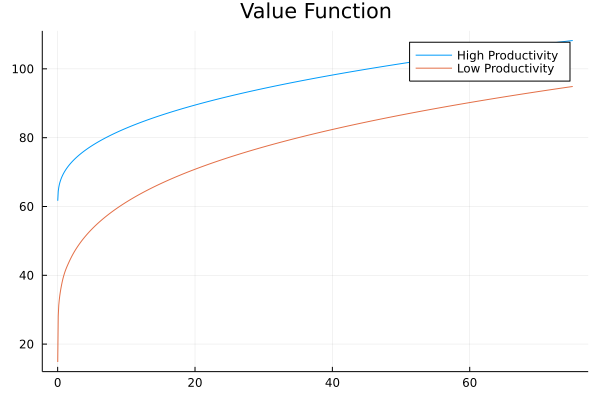
\includegraphics[width=.8\linewidth]{./julia/figure_valfunc_julia.png}
	\end{center}
\end{itemize}

\pagebreak

\section{}

\begin{itemize}
\item The decision rule is increasing in $k$ and $z$ (i.e., $K'(k_{i+1},z)\ge K'(K_{i},z)$). Also, saving is increasing in $z$ (i.e., $k'(k,z)-k$ is increasing in $z$). With regard to $k$, in $z_{g}$ saving is first increasing but turns to be decreasing, whereas in $z_{b}$ saving is always decreasing. My argument is presented in the below two figures.
\begin{center}
	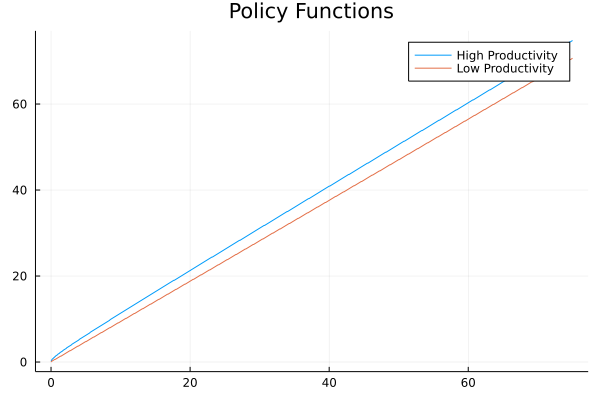
\includegraphics[width=.8\linewidth]{./julia/figure_polfunc_julia.png}
\end{center}
\begin{center}
	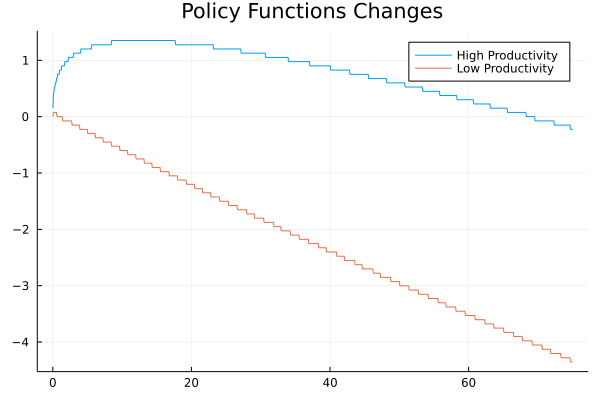
\includegraphics[width=.8\linewidth]{./julia/figure_polfuncdiff_julia.png}
\end{center}

\pagebreak

\item Also, figures drawn from Fortran and Matlab are presented below.
\begin{enumerate}
	\item \textbf{Fortran}
	\begin{center}
		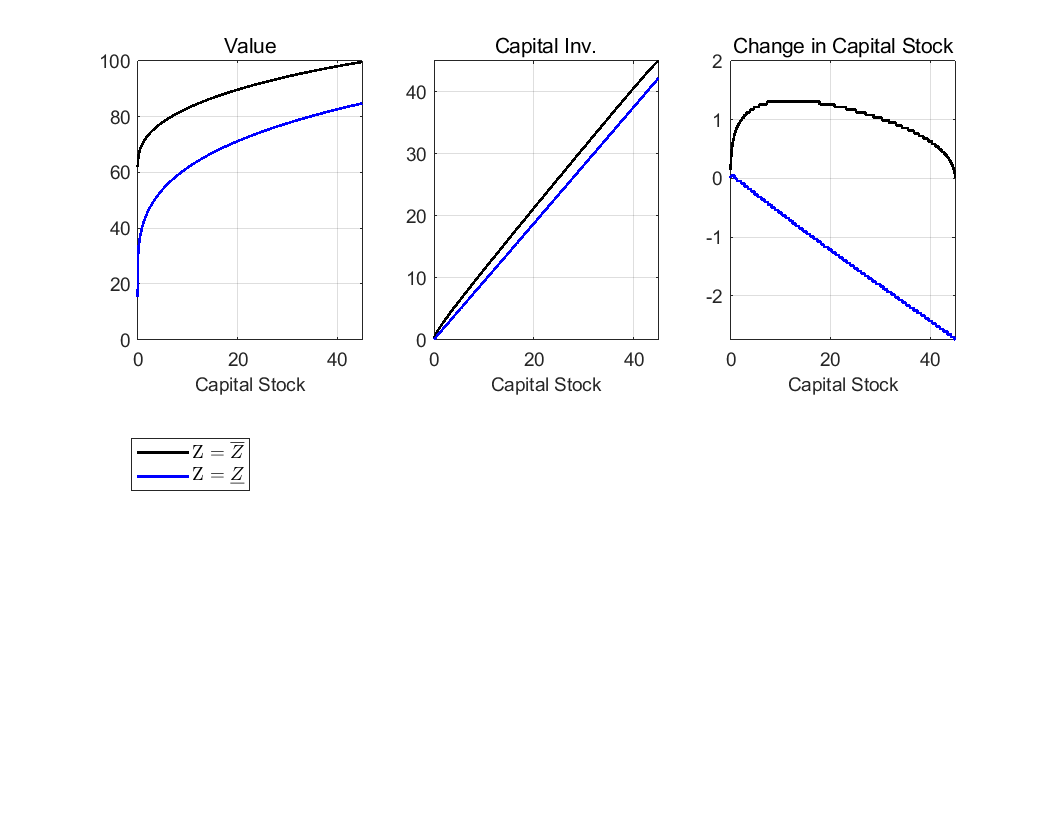
\includegraphics[width=1\linewidth]{./fortran/figure_fortran.png}
	\end{center}
	\item \textbf{Matlab}
	\begin{center}
		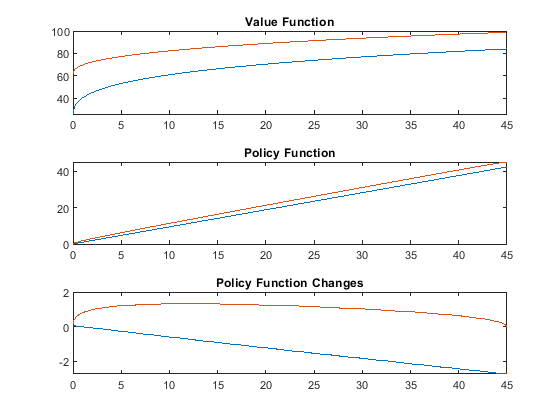
\includegraphics[width=1\linewidth]{./matlab/figure_matlab.png}
	\end{center} 
\end{enumerate}
\end{itemize}

	
\end{document}